\documentclass[12pt]{article}
\usepackage{epsf}
\usepackage{amsmath,amssymb}

\usepackage{graphicx}

\usepackage{comment}
\usepackage{listings}
\usepackage{hyperref}

\setlength{\textwidth}{16.5cm}
\setlength{\textheight}{21.5cm}
\setlength{\oddsidemargin}{0cm}
\setlength{\evensidemargin}{0cm}
\setlength{\topmargin}{0cm}
\setlength{\footskip}{1cm}

\renewcommand{\topfraction}{1.0}
\renewcommand{\bottomfraction}{1.0}

\begin{document}

\newcommand{\lsim}{\stackrel{<}{_\sim}}
\newcommand{\gsim}{\stackrel{>}{_\sim}}
%\newcommand{\mathhyphen}{\mathchar"712D}

\newcommand{\codename}{{\tt ELVAS}\, }

\newcommand{\rem}[1]{{$\spadesuit$\bf #1$\spadesuit$}}

%\renewcommand{\theequation}{\thesection.\arabic{equation}}

\renewcommand{\thefootnote}{\fnsymbol{footnote}}
\setcounter{footnote}{0}

\begin{titlepage}

\begin{center}

\hfill Updated Oct. 2024

\vskip .5in

{\Large\bf
{\LARGE \codename}\\[3mm]
C++ Package for ELectroweak VAcuum Stability\\
}
\vskip .1in
S. Chigusa, T. Moroi, and Y. Shoji

\end{center}


\vspace{0.3\textheight}


\end{titlepage}

\setcounter{page}{1}
\renewcommand{\thefootnote}{\#\arabic{footnote}}
\setcounter{footnote}{0}

\section{Introduction}

\codename is a C++ package for the calculation of the decay rate of a
false vacuum at the one-loop level, based on the formulae developed in
\cite{Chigusa:2017dux, Chigusa:2018uuj}. The degeneracy of the gauge transverse modes is corrected according to \cite{Baratella:2024hju}.

\codename is applicable to models with
the following features:
\begin{itemize}
\item Only one scalar boson is responsible for the vacuum decay.
\item Classical scale invariance (approximately) holds.  In
  particular, the potential of the scalar field responsible for the
  vacuum decay should be well approximated by the quartic form for
  the calculation of the bounce solution.  (Thus, the bounce is
  nothing but the so-called Fubini instanton.)
\item The instability of the scalar potential occurs due to RG
  effects; thus, the quartic coupling constant becomes negative at a
  high scale.
\end{itemize}

If you use \codename in scholarly work, please cite
\cite{Chigusa:2017dux}, \cite{Chigusa:2018uuj} and \cite{Baratella:2024hju}.

\section{Setup}

We denote the (complex) scalar field responsible for the vacuum decay
as $\Phi$.  Then, \codename assumes that the scalar potential is given
in the following form:
\begin{align}
  V(\Phi) = \lambda(\Phi^\dagger\Phi)^2,
  \label{pot}
\end{align}
where $\lambda$ is a coupling constant.  The instability occurs due to
the renormalization group (RG) running of $\lambda$; $\lambda$ is
positive at a low scale while is negative at a high scale due to RG
effect.

The Higgs may interacts with other (real) scalar field $\sigma$ and
chiral fermions $\psi_L$ and $\psi_R$.  The interaction terms are
denoted as
\begin{align}
  {\cal L}_{\rm int} = \kappa \sigma^2 \Phi^\dagger\Phi
  + (y \Phi \psi_L \psi_R + {\rm h.c.}),
\end{align}
where $\kappa$ and $y$ are coupling constants.  

The scalar field $\Phi$ may also have gauge interaction.  The ``gauge
coupling constant'' in this package is defined such that the
corresponding gauge boson mass is given by
\begin{align}
  m_A^2=2g^2\langle\Phi^\dagger\Phi\rangle.
\end{align}
where the brackets indicate the vacuum expectation value.

For a negative $\lambda$, we have the Fubini instsanton, which is given by
\begin{equation}
 \bar\phi(r) =
 \sqrt{\frac{8}{|\lambda|}}\frac{1}{R}
 \left(
  1+\frac{r^2}{R^2}
 \right)^{-1},
\end{equation}
where $\bar\phi = \sqrt{\langle\Phi^\dagger\Phi\rangle / 2}$, $r$ is the
distance from the center of the instanton, and $R$ is a constant
determining the size of the instanton. We denote the field value at the
center of the instanton as $\bar\phi_C$, which is related to $R$ by
\begin{equation}
 \bar\phi_C=\sqrt{\frac{8}{|\lambda|}}\frac{1}{R}.
\end{equation}

The decay rate with a pair of chiral fermions, a scalar field and a
$U(1)$ gauge field is then expressed as
\begin{align}
 \gamma &=
 \int d\ln R^{-1}\frac{\mathcal V_G}{R^4}
 \left[
  \mathcal A'^{(h)}\mathcal A^{(\sigma)}\mathcal A^{(\psi)}
  \mathcal A'^{(A,\varphi)} e^{-\mathcal B}
 \right]_{\rm \overline{MS},\mu\sim1/R}\nonumber\\
 &\equiv
 \int d\ln R^{-1}\exp
 \left[
  \ln\frac{d\gamma}{d\ln R^{-1}}
 \right],
\end{align}
where $\mathcal V_G$ is the volume of the group space generated by the
broken generators, $\mathcal B$ is the tree level action of the
instanton, and $\mathcal A^{(X)}$ is the quantum correction from
particle $X$. The coupling constants and quantum corrections are
renormalized in $\rm \overline{MS}$-scheme, and the renormalization
scale, $Q$, is taken so that $Q\sim 1/R$ to handle possible large
logarithmic corrections.  Notice that $\mathcal V_G$, has to be measured
with ``$U(1)$'' generators. For the SM or its extensions only with
scalars and fermions, it is $2\pi^2$. If $\Phi$ has only a U(1)
charge, it is $2\pi$.

This package first calculates $\ln\frac{d\gamma}{d\ln R^{-1}}$ for each
$\ln R^{-1}$, using a renormalization group data provided by user.  Then,
it interpolates $\ln\frac{d\gamma}{d\ln R^{-1}}$ and integrates
$\frac{d\gamma}{d\ln R^{-1}}$.
\section{Download and install}
To use \codename, you need a
\verb|c++| compiler that supports C++14, and the \verb|boost| library.
The required version of \verb|boost| is 1.59.0\footnote{We found that {\tt boost 1.58.0} has a serious bug.}. 
\subsection{Unix}
For UNIX systems, follow the instruction below.
\begin{enumerate}
 \item Clone the \codename git repository
\begin{lstlisting}[basicstyle=\ttfamily\footnotesize, frame=single]
 git clone https://github.com/YShoji-HEP/ELVAS.git
\end{lstlisting}
Or, you can download it from \href{https://github.com/YShoji-HEP/ELVAS/}{https://github.com/YShoji-HEP/ELVAS/}.
 \item Generate a makefile with
\begin{lstlisting}[basicstyle=\ttfamily\footnotesize, frame=single]
 cmake .
\end{lstlisting}
If you do not use the default compiler, use
\begin{lstlisting}[basicstyle=\ttfamily\footnotesize, frame=single]
-DCMAKE_CXX_COMPILER=your++
\end{lstlisting}
option. When the \verb|boost| library is located at a non-standard
       directory, specify it with
\begin{lstlisting}[basicstyle=\ttfamily\footnotesize, frame=single]
-DBOOST_ROOT=/your/dir
\end{lstlisting}
or
\begin{lstlisting}[basicstyle=\ttfamily\footnotesize, frame=single]
-DBOOST_INCLUDEDIR=/your/inc -DBOOST_LIBRARYDIR=/your/lib
\end{lstlisting}
If you have installed the google perftools, you can enable
       \verb|tcmalloc| with
\begin{lstlisting}[basicstyle=\ttfamily\footnotesize, frame=single]
-DUSE_TCMALLOC=ON
\end{lstlisting}
 \item Compile \codename with
\begin{lstlisting}[basicstyle=\ttfamily\footnotesize, frame=single]
 make
\end{lstlisting}
 \item Run
\begin{lstlisting}[basicstyle=\ttfamily\footnotesize, frame=single]
 ./elvas sm.in sm.dat
\end{lstlisting}
If everything works well, you will see as a result
\begin{lstlisting}[basicstyle=\ttfamily\footnotesize, frame=single]
mHiggs       mTop         log10(gamma x Gyr Gpc^3)
1.250900e+02 1.731000e+02 -5.796066e+02
1.248500e+02 1.731000e+02 -5.396598e+02
1.253300e+02 1.731000e+02 -6.242081e+02
1.250900e+02 1.725000e+02 -9.053941e+02
1.250900e+02 1.737000e+02 -3.968497e+02
\end{lstlisting}
after a header.
\end{enumerate}
If you have link errors, check the summary of
\verb|cmake| and make sure it finds a correct version of \verb|boost|.

If you are not using the default compiler, the installed \verb|boost|
library may not be compiled with your compiler. In such a case, you need
to use the default compiler or compile \verb|boost| with \verb|toolset|
option. Make sure that a path to dynamic library files is correctly
added to the environment variable if you use a dynamic library.

From
\verb|boost 1.66.0|, library filenames may contain the system architecture tag, {\it e.g.} \verb|-x32|, but it seems that \verb|cmake 3.11.0-rc1|
does not support the tag. In such a case, make symbolic links for
\verb|boost_system| and \verb|boost_program_options| so that they do not
contain the tag.
\subsection{Windows}
For Windows, you may use
\verb|Cygwin|, \verb|MinGW|, or \verb|Visual C++|.  In any case, you
need to install \verb|cmake|, which can be downloaded from the official
website.  For \verb|Cygwin| and \verb|MinGW|, the procedure is almost
the same as the UNIX systems.  For
\verb|Visual C++|, you can generate a VC++ project file with the GUI front-end of \verb|cmake|.
Furthermore, a pre-compiled
\verb|boost| library can be installed through \verb|NuGet|. After
installing it, you can build the project as usual.

\section{How to use \codename}

\codename provides routines for the calculation of a decay rate together
with an interpreter. The easiest way to use this program is to use the
interpreter, but you may directly call the routines in your {\tt c++}
code.
\subsection{Quick guide to use interpreter}
The easiest way to calculate vacuum decay rates in your model is to modify
\verb|sm.in|, which is provided in the package.
\begin{enumerate}
 \item Copy \verb|sm.in| so that you can resume the original input file
       when something goes wrong.  (We name the copied file
       \verb|model.in| in this guide.)
 \item Calculate the RG evolution of the couplings in your model. It is
       preferable to use, at least, two-loop beta functions for the
       running. The interval of the data points should be short enough;
       about five points between $Q$ and $10Q$ is enough. If you limit
       the region of integration, the RG data should cover all the
       region. If you do not limit the region, you need to solve the RG
       equations until the Higgs quartic coupling becomes positive
       again. Since this package does not provide any solver of
       differential equations, you need to solve them by yourself.
 \item Format the RG data as follows. (We name this file \verb|rg.dat| in
       this guide.)

\begin{lstlisting}[basicstyle=\ttfamily\footnotesize, frame=single]
[DATASET] (1.20000e+02 1.70000e+02)
2.40000e+02 6.45699e-01 4.62621e-01 9.00513e-01 ... 
3.80374e+02 6.43314e-01 4.63832e-01 8.78139e-01 ... 
...
[DATASET] (1.20000e+02 1.70200e+02)
...
\end{lstlisting}
       The statement of \verb|[DATASET]| indicates the beginning
       of a ``dataset''. The numbers in parentheses are ``dataset
       variables'', which are optional common variables for the
       dataset. If you do not provide any dataset variables, you can omit
       the parentheses and just
       \verb|[DATASET]| is enough. Each row below the \verb|[DATASET]|
       statement is a ``record'' that belongs to the dataset. A record
       should contain information about the renormalization scale and
       the values of coupling constants at the scale. The dataset ends
       when it reaches the end of file or a new \verb|[DATASET]|
       statement. You may use several formats for numbers like
       \verb|1|, \verb|1.2|, \verb|1.23e10| and \verb|2.E-10|.  If you
       want to use different delimiters, modify
       \verb|DATASET_DELIM| and \verb|RECORD_DELIM| in the \verb|[GENERAL]|
       section.
 \item Label the dataset variables. It can be done with
       \verb|DATASET_VARS| in the \verb|[GENERAL]| section.
       It looks like
\begin{lstlisting}[basicstyle=\ttfamily\footnotesize, frame=single]
DATASET_VARS = {mHiggs, mTop}
\end{lstlisting}
       The names should be comma-separated and be in braces.  Make
       sure that the order is the same as the entries in \verb|rg.dat|.
       You can use alphabets, numbers and underscore for the name, but
       it cannot start with a number. If you do not provide any dataset
       variables, set \verb|DATASET_VARS = {}|.
 \item Label the values in a record with
       \verb|RECORD_VARS| in the \verb|[GENERAL]| section, similarly as
       dataset variables. It looks like
\begin{lstlisting}[basicstyle=\ttfamily\footnotesize, frame=single]
RECORD_VARS = {Q, g2, g1, yt, yb, lambda}
\end{lstlisting}
 \item Set the ratio between the renormalization scale, $Q$, and the
       instanton scale, $R^{-1}$. It can be set by the following entry
       in the \verb|[INITIALIZE]| section.
\begin{lstlisting}[basicstyle=\ttfamily\footnotesize, frame=single]
LN_QR = 0
\end{lstlisting}
       The above entry sets $\ln QR=0$, {\it i.e.}, $Q=R^{-1}$.
 \item Set the volume of the group space generated by the broken
       generators, $\ln \mathcal V_G$. It can be set with the following
       entry in the \verb|[INITIALIZE]| section.
\begin{lstlisting}[basicstyle=\ttfamily\footnotesize, frame=single]
lnVg = log(2. * pi^2)
\end{lstlisting}
 \item Set an upper bound on the region of integration over $\ln
       R^{-1}$. You can find the following entry in the
       \verb|[INITIALIZE]| section.
\begin{lstlisting}[basicstyle=\ttfamily\footnotesize, frame=single]
upper_bound = log(2.435e18)
\end{lstlisting}
      It sets upper bounds both on $\ln R^{-1}$ and $\ln\bar\phi_C$. The
       integral stops when either of these becomes larger than the
       Planck scale in the above example.

\item Set a lower bound on the region of integration over $\ln R^{-1}$.
\begin{lstlisting}[basicstyle=\ttfamily\footnotesize, frame=single]
lower_bound = log(mTop * 10)
\end{lstlisting}
       It sets lower bounds both on $\ln R^{-1}$ and $\ln\bar\phi_C$. The
       integral starts when both of these becomes ten times larger than
       the top mass in the above example. This line is in the
       \verb|[BEGIN_ROUTINE]| section because it uses a dataset variable,
       \verb|mTop|. If you do not use any dataset variables in this line,
       you may move it to the \verb|[INITIALIZE]| section.
 \item In the following entry in the \verb|[MAIN_ROUTINE]| section,
       describe the Higgs quartic coupling that is normalized as in
       eq.~\eqref{pot}.
\begin{lstlisting}[basicstyle=\ttfamily\footnotesize, frame=single]
HIGGS_QUARTIC_COUPLING = lambda
\end{lstlisting}
       You can use the variables in
       \verb|DATASET_VARS| and \verb|RECORD_VARS|.  If needed, you can
       normalize it in this line like
       \verb|HIGGS_QUARTIC_COUPLING = lambda / 2|.
 \item In the following entry in the \verb|[MAIN_ROUTINE]| section,
       describe the instanton scale, $\ln R^{-1}$, using \verb|LN_QR|
       and the variables in \verb|DATASET_VARS| and \verb|RECORD_VARS|.
\begin{lstlisting}[basicstyle=\ttfamily\footnotesize, frame=single]
LN_RINV = log(Q) - LN_QR
\end{lstlisting}
 \item In the following entries in the \verb|[MAIN_ROUTINE]| section,
       set \verb|totalQC| and \verb|maxQC|, which
       are $\sum_X[-\ln\mathcal A^{(X)}]_{\rm \overline{MS}}$ and
       $\max_X|[-\ln\mathcal A^{(X)}]_{\rm \overline{MS}}|$, respectively.
\begin{lstlisting}[basicstyle=\ttfamily\footnotesize, frame=single]
higgsQC = HiggsQC()
topQC = 3. * FermionQC(yt)
WbosonQC = 2. * GaugeQC(g2^2 / 4.)
ZbosonQC = GaugeQC((g2^2 + g1^2 * 3. / 5.) / 4.)

totalQC = higgsQC + topQC + WbosonQC + ZbosonQC
maxQC = max(abs(topQC), abs(WbosonQC), abs(ZbosonQC), abs(higgsQC))
\end{lstlisting}
Here, you may use
       \verb|HiggsQC()|, \verb|ScalarQC(kappa)|, \verb|FermionQC(y)|, and \verb|GaugeQC(g_squared)|
       to calculate $[-\ln\mathcal A^{(X)}]_{\rm \overline{MS}}$ of
       the Higgs field, a scalar field with $\kappa=$
       \verb|kappa|, a pair of chiral fermions with $y=$ \verb|y|, and a $U(1)$ gauge field with $g^2=$ \verb|g_squared|,
       respectively.
 \item List up what you want to print on the output file.
\begin{lstlisting}[basicstyle=\ttfamily\footnotesize, frame=single]
print(mHiggs, mTop, (lngamma + 378.229) / log(10))
\end{lstlisting}
       Here, \verb|lngamma| is $\ln\gamma$, where $\gamma$ is given in
       the same unit as $R^{-4}$. The delimiter can be set with
       \verb|OUTPUT_DELIM| in the \verb|[GENERAL]| section.  You may
       optionally print a header by modifying
\begin{lstlisting}[basicstyle=\ttfamily\footnotesize, frame=single]
print("mHiggs       mTop         log10(gamma x Gyr Gpc^3)")
\end{lstlisting}
       in the \verb|[INITIALIZE]| section. You may change the decimal
       precision for the output with \verb|output_precision(n)|, which
       should be put in the \verb|[INITIALIZE]| section.
 \item Execute the program by typing
\begin{lstlisting}[basicstyle=\ttfamily\footnotesize, frame=single]
./elvas -o result.out model.in rg.dat
\end{lstlisting}
       in a terminal.
       The result will be written to \verb|result.out|.
       
       You may provide multiple input files, which will be joined internally.
       Allowed options are
       \begin{description}
	\item[-o] output file
	\item[-h] display help message
        \item[-v] output version information
        \item[-n] disable header printing
       \end{description}
       If input/output file is not supplied, the program use the
       standard input/output.
\end{enumerate}

\subsection{Using interpreter}
The input of the interpreter has the following sections:
\verb|[GENERAL]|, \verb|[INITIALIZE]|, \verb|[BEGIN_ROUTINE]|,
\verb|[MAIN_ROUTINE]|, \verb|[END_ROUTINE]|, \verb|[FINALIZE]| and zero
or more \verb|[DATASET]|'s. You can omit any sections if you do not use
them.  As shown in the flowchart (Fig.~\ref{flow}), the interpreter
first reads
\verb|[GENERAL]| and recognize the formats used in \verb|[DATASET]| and
output. Then, it executes
\verb|[INITIALIZE]|. When the \verb|[DATASET]| section begins, \verb|[BEGIN_ROUTINE]|
is executed. At each record in the \verb|[DATASET]| section,
\verb|[MAIN_ROUTINE]| is executed. After all the record in \verb|[DATASET]|
are evaluated, \verb|[END_ROUTINE]| is executed and the interpreter will
search for the next
\verb|[DATASET]| section. After all \verb|[DATASET]|'s are evaluated,
\verb|[FINALIZE]| is executed and the program terminates.

\begin{figure}[t]
 \begin{center}
  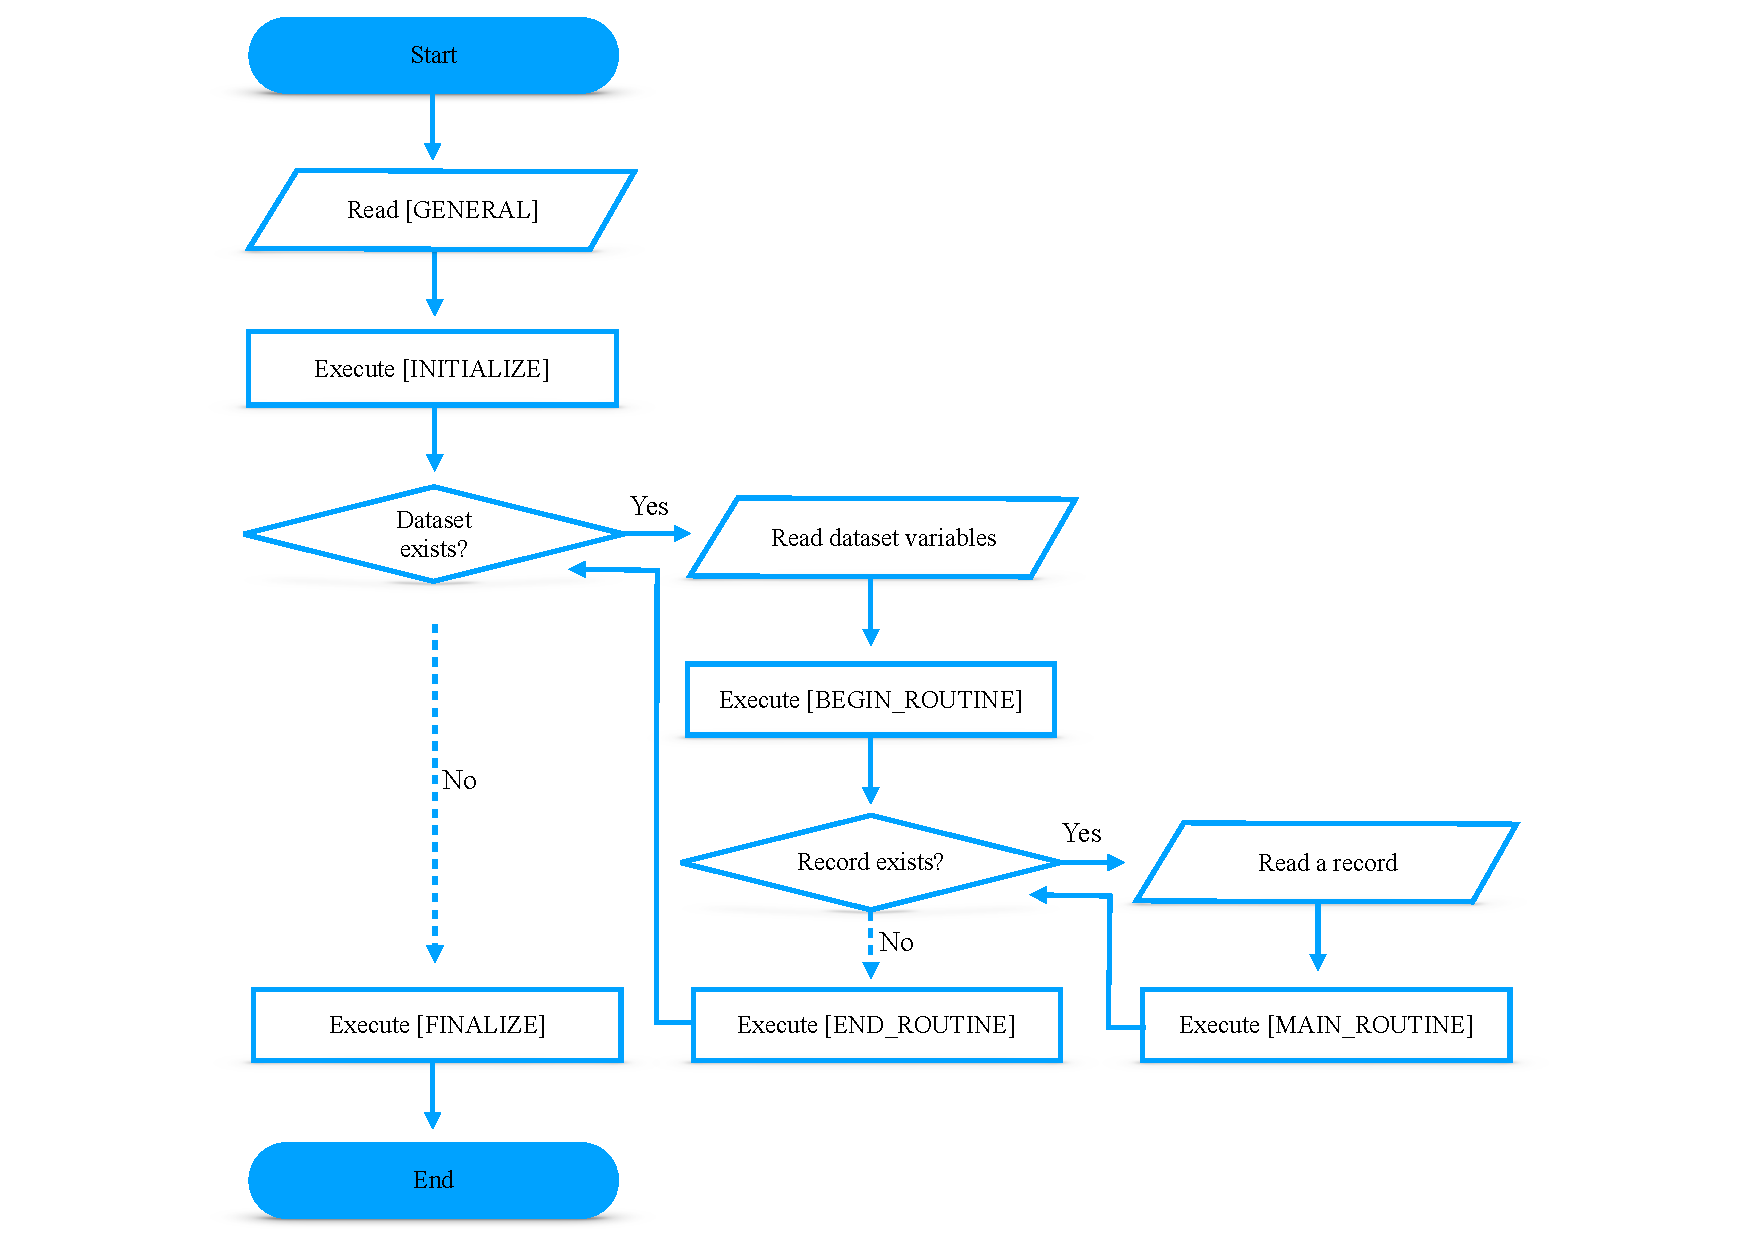
\includegraphics[width=0.8\linewidth]{flowchart.pdf}
 \end{center}
 \caption{The flowchart of the interpreter.}
 \label{flow}
\end{figure}

The details of \verb|[DATASET]| can be found in the previous
subsection and those of the others are given below.
\subsubsection*{Section \tt [GENERAL]}
This section is for general settings. It should appear first in an
input file if you use it. 

If you have one or more dataset variables, you need to set
\begin{itemize}
 \item \verb|DATASET_DELIM = "delim"| -- The delimiter for dataset variables.
 \item \verb|DATASET_VARS = {dataset_var_name1, dataset_var_name2, ...}| -- The names for dataset variables. You can use alphabets, numbers and underscore, but a name cannot start with a number. If you have no dataset variables, set it to \verb|{}|.
\end{itemize}
If you have one or more records, you need to set
\begin{itemize}
 \item \verb|RECORD_DELIM = "delim"| -- The delimiter for records.
 \item \verb|RECORD_VARS = {data_var_name1, data_var_name2, ...}| -- The names for variables in a record. You can use alphabets, numbers and underscore, but a name cannot start with a number.
\end{itemize}

If you output numbers, you need to set
\begin{itemize}
 \item \verb|OUTPUT_DELIM = "delim"| -- The delimiter for output.
\end{itemize}

\subsubsection*{Section \tt [INITIALIZE] [BEGIN\_ROUTINE]
[MAIN\_ROUTINE] [END\_ROUTINE] [FINALIZE]}

In these sections, you can make your own routine with a simple grammar.
We first list basic specifications.
\begin{itemize}
 \item Input
\begin{itemize}
 \item The routine is evaluated line by line. If you want to do a line
       break, put \verb|\| before you start a new line.
 \item White spaces and tabs are ignored.
 \item Any characters after \verb|#| are ignored.
\end{itemize}
 \item Basic calculation
\begin{itemize}
 \item You may use
       \verb|+|, \verb|-|, \verb|*|, \verb|/|, and \verb|^|, for  addition, subtraction, multiplication, division, and power, respectively. You may use \verb|pow(x,y)|, instead of \verb|x^y|. If \verb|y| is integer, \verb|x^y| is faster than \verb|pow(x,y)|.
 \item For relational operators, you may use
       \verb|<|, \verb|>|, \verb|<=|, \verb|>=|, \verb|==|, and \verb|!=|,
       which correspond to $<$, $>$, $\leq$, $\geq$, $=$, and $\neq$,
       respectively. If the result is true, it returns one, otherwise it
       returns zero. Since numbers are processed as
       \verb|double|, it is not preferred to use \verb|x == y|. Instead, you may
       use \verb|abs(x-y) < some_small_number|.
 \item You may combine the relational conditions by using \verb|&| and \textbar~as ``and'' and ``or'' operators, respectively.
 \item Parentheses, ``\verb|(|'' and ``\verb|)|'', can be used to group expressions.
 \item Constant $\pi$ is defined as \verb|pi|.
\end{itemize}
\item Functions
\begin{itemize}
 \item You may use the following elementary functions: \verb|pow(x,y)|, \verb|abs(x)|,
       \verb|sqrt(x)|, \verb|exp(x)|, \verb|log(x)|, \verb|log10(x)|, \verb|sin(x)|, \verb|cos(x)|, \verb|tan(x)|, \verb|asin(x)|, \verb|acos(x)|, and \verb|atan(x)|. Make sure that the result is always real.
 \item The maximum and the minimum value can be obtained with
       \verb|max(x,y,...)| and \verb|min(x,y,...)|, respectively. The
       number of arguments should be equal or larger than two.
\end{itemize}
\item Definition of constants and functions
\begin{itemize}
 \item You may define a constant with
       \verb|=| operator. For example, \verb|c = 2 * 3| sets 6 to \verb|c|. You
       can use alphabets, numbers and underscore for the name of a
       constant, but it cannot start with a number. It returns the
       result of the right-hand side. Once it is defined, it remains
       until the program terminates.
 \item You may define a function with
       \verb|:=| operator. For example, \verb|f(x):=x^2| defines a
       function \verb|f(x)| that returns the square of \verb|x|.  You
       can use alphabets, numbers and underscore for the name of a
       function, but it cannot start with a number. Once it is defined,
       it remains until the program terminates. If the number of
       arguments is zero, you can define it either by
       \verb|g():=...| or by \verb|g:=...|, and call it either by \verb|g()|
       or by \verb|g|. (When there is a confliction between the names of
       a constant and a function, the constant overrides the function.)
 \item It is allowed to use
       \verb|:=| and multiple \verb|=|'s at the same time. For example, 
       \verb|f(x):=m=x^2| sets the result of $x^2$ to \verb|m|
       when it is evaluated. 
\end{itemize}
\item Utilities
\begin{itemize}
  \item Conditional branches can be expressed with
       \verb|if(cond, x)| or \verb|if(cond, x, y)|. If \verb|cond| is equal or larger than $0.5$, only \verb|x| is evaluated and returns the result, otherwise only \verb|y| is evaluated and returns the result. If \verb|y|
       is not provided and
       \verb|cond| is less than $0.5$, it returns zero without evaluating \verb|x|.
 \item You may evaluate multiple expressions at the same time with
      \verb|eval(expr1, expr2, ...)|. You can use any operators except
      for \verb|:=| in the arguments. It returns the result of the last
      argument.
 \item If you want to skip the rest of the entries in a section, use \verb|continue()|.
 \item If you want to skip a dataset, use \verb|break()|. Once it is
       called, the interpreter skips the rest of the records in the current
       \verb|[DATASET]| section and the coming \verb|[END_ROUTINE]| section.
 \item If \verb|exit()| is called, the program terminates.
\end{itemize}
\item Output
\begin{itemize}
 \item \verb|print("string")| function prints \verb|string| on the output file.
 \item \verb|print(num1, num2, ...)| function prints numbers on the
       output file.  The delimiter can be set with the
       \verb|OUTPUT_DELIM| entry in the \verb|[GENERAL]| section. It
       returns the result of the last argument.
 \item \verb|output_precision(n)| sets the decimal precision for output to \verb|n|.
\end{itemize}
\end{itemize}

In addition, there are constants and functions used for the calculation
of vacuum decay rates. They should be set or called in right places.
\begin{itemize}
 \item[$\blacksquare$] In section \verb|[INITIALIZE]|
\begin{description}
 \item[const] \verb|LN_QR| -- It fixes $\ln QR$, which should be
       a constant and relates the renormalization scale, $Q$, and the
       instanton scale, $R$.
\end{description}
 \item[$\blacksquare$] In section \verb|[BEGIN_ROUTINE]|
\begin{description}
 \item[func] \verb|initialize()| -- It clears the accumulated data of $\ln\bar\phi_C$ and
      $\ln d\gamma/dR^{-1}$. If you have multiple \verb|[DATASET]|'s, this
       function must be called.
\end{description}
 \item[$\blacksquare$] In section \verb|[MAIN_ROUTINE]|
\begin{description}
 \item[const] \verb|HIGGS_QURTIC_COUPLING| -- The Higgs quartic coupling
	      normalized as in eq.~\eqref{pot}.
 \item[const] \verb|LN_RINV| -- The instanton scale, $\ln R^{-1}$.
 \item[func]  \verb|InstantonB()| -- It returns the tree level action,
              $\mathcal B$. \verb|HIGGS_QUARTIC_COUPLING|
             should be set before this function is called.
 \item[func] \verb|HiggsQC()| -- It returns the quantum corrections 
             from the Higgs fluctuations,
             $\left[-\ln\mathcal A^{(h)}\right]_{\rm \overline{MS}}$.
             \verb|HIGGS_QUARTIC_COUPLING| and \verb|LN_QR|
             should be set before this function is called.
 \item[func] \verb|ScalarQC(kappa)| -- It returns the quantum corrections
             from the scalar fluctuations, 
             $\left[-\ln\mathcal A^{(\sigma)}\right]_{\rm \overline{MS}}$
             with $\kappa=$ \verb|kappa|. \verb|HIGGS_QUARTIC_COUPLING| 
             and \verb|LN_QR| should be set before this function is called.
  \item[func] \verb|FermionQC(y)| -- It returns the quantum corrections from
               the fermion fluctuations, 
              $\left[-\ln\mathcal A^{(\psi)}\right]_{\rm \overline{MS}}$ with
              $y=$ \verb|y|. \verb|HIGGS_QUARTIC_COUPLING| and \verb|LN_QR|
              should be set before this function is called.
  \item[func] \verb|GaugeQC(g_squared)| -- It returns the quantum corrections
              from the gauge fluctuations, $\left[-\ln\mathcal
	      A^{(A,\varphi)}\right]_{\rm \overline{MS}}$ with $g^2=$
	      \verb|g_squared|. \verb|HIGGS_QUARTIC_COUPLING| and \verb|LN_QR|
              should be set before this function is called.
  \item[func] \verb|save_phiC()| -- It saves $\ln\bar\phi_C$ to
	      memory. If you use
              \verb|get_max_lnQ(x)| or \verb|get_min_lnQ(x)|, you need
              to execute this
	      function. \verb|HIGGS_QURTIC_COUPLING| and 
              \verb|LN_RINV| should be set before this function is called.
  \item[func] \verb|save_dlngamma_dRinv(dlngamma)| -- It saves 
              $\ln d\gamma/dR^{-1}=$ \verb|dlngamma| to memory. If you use
              \verb|get_lngamma(x,y)|, you need to execute this function. 
              \verb|LN_RINV| should be set before this function is called.
\end{description}
  \item[$\blacksquare$] In section \verb|[END_ROUTINE]|
 \begin{description}
  \item[func] \verb|is_data_enough()| -- It checks if there are enough
              data points of $\ln d\gamma/dR^{-1}$ to calculate the
              decay rate. It returns one if they are enough, or zero if
	      not.
  \item[func] \verb|get_max_lnRinv(upper_bound)| -- It returns the maximum
              allowed value of $\ln R^{-1}$ where both $\ln\bar\phi_C$ and
	      $\ln R^{-1}$ are
              below \verb|upper_bound|. If all the saved data points have
	      smaller $\ln R^{-1}$, it returns the maximum $\ln R^{-1}$
	      among the data points.
  \item[func] \verb|get_min_lnRinv(lower_bound)| -- It returns the
	      minimum allowed
              value of $\ln R^{-1}$ where both $\ln \bar\phi_C$ and 
              $\ln R^{-1}$ are
              above \verb|lower_bound|. If all the saved data points have
	      larger $\ln R^{-1}$, it returns the minimum $\ln R^{-1}$
	      among the data points.
  \item[func] \verb|get_lngamma(lnRinv_min,lnRinv_max)| -- It
              interpolates the accumulated $\ln d\gamma/dR^{-1}$ and
              integrates over interval
              [\verb|lnRinv_min|,\verb|lnRinv_max|]. The return value is
	      $\ln \gamma$. There should be a sufficient number of saved data
	      that cover the region of integration.
 \end{description}
\end{itemize}

\subsection{Call routines in a {\tt c++} code}
If you use our routines in your
\verb|c++| code, include \verb|elvas.h| and compile \verb|elvas.cpp|
together with your code. The following routines are defined. They do not
require the \verb|boost| library.
\begin{itemize}
 \item \verb|Elvas::instantonB(lambdaAbs)|

Calculate the tree level action of the instanton.
\begin{description}
 \item[in] \verb|const double& lambdaAbs|

 The value of $|\lambda |$.
 \item[out] The value of tree level action, $\mathcal B$.
\end{description}
 \item \verb|Elvas::higgsQC(lambdaAbs, lnQR)|

Calculate the quantum corrections from the Higgs field.
\begin{description}
 \item[in] \verb|const double& lambdaAbs|

 The value of $|\lambda |$.
 \item[in] \verb|const double& lnQR|

 The value of $\ln Q R$.
 \item[out] The value of $\left[-\ln\mathcal A'^{(h)}\right]_{\rm \overline{MS}}$.
\end{description}
 \item \verb|Elvas::scalarQC(kappa, lambdaAbs, lnQR)|

Calculate the quantum corrections from a scalar.
\begin{description}
 \item[in] \verb|const double& kappa|

 The value of $\kappa$.
 \item[in] \verb|const double& lambdaAbs|

 The value of $|\lambda |$.
 \item[in] \verb|const double& lnQR|

 The value of $\ln Q R$.
 \item[out] The value of $\left[-\ln\mathcal A^{(\sigma)}\right]_{\rm \overline{MS}}$.
\end{description}
 \item \verb|Elvas::fermionQC(y, lambdaAbs, lnQR)|

Calculate the quantum corrections from a pair of chiral fermions.
\begin{description}
 \item[in] \verb|const double& y| 

The value of $y$.
 \item[in] \verb|const double& lambdaAbs| 

The value of $|\lambda |$.
 \item[in] \verb|const double& lnQR| 

The value of $\ln Q R$.
 \item[out] The value of $\left[-\ln\mathcal A^{(\psi)}\right]_{\rm \overline{MS}}$.
\end{description}
 \item \verb|Elvas::gaugeQC(gSquared, lambdaAbs, lnQR)|

Calculate the quantum corrections from a $U(1)$ gauge boson.
\begin{description}
 \item[in] \verb|const double& gSquared| 

The value of $g^2$.
 \item[in] \verb|const double& lambdaAbs| 

The value of $|\lambda |$.
 \item[in] \verb|const double& lnQR| 

The value of $\ln Q R$.
 \item[out] The value of $\left[-\ln\mathcal A^{(A,\varphi)}\right]_{\rm \overline{MS}}$.
\end{description}
 \item \verb|Elvas::lnPhiC2LnRinv(lnPhiC, lnPhiC2lnRinv)|

Convert $\ln\bar\phi_C$ to $\ln R^{-1}$.
\begin{description}
 \item[in] \verb|const double& lnPhiC| 

The value of $\ln\bar\phi_C$.
 \item[in, out] \verb|vector<pair<double, double>>&lnPhiC2lnRinv| 

A vector of $(\ln\bar\phi_C,\ln R^{-1})$.
 \item[out] 

The corresponding value of $\ln R^{-1}$.
\end{description}
 \item \verb|Elvas::getLnGamma(lndgam, lnRinvBeg, lnRinvEnd)|

Integrate over $\ln R^{-1}$, using accumulated data of $\ln\frac{d\gamma}{d\ln R^{-1}}$.
\begin{description}
 \item[in, out] \verb|vector<pair<double, double>>& lndgam| 

A vector of $\left(\ln R^{-1},\ln\frac{d\gamma}{d\ln R^{-1}} \right)$.
 \item[in] \verb|const double& lnRinvBeg| 

The lower boundary of the region of integration.
 \item[in] \verb|const double& lnRinvEnd| 

The upper boundary of the region of integration.
 \item[out] The value of $\ln\gamma$.
\end{description}
\end{itemize}
\appendix
\section{Example model file}
\begin{lstlisting}[basicstyle=\ttfamily\footnotesize, frame=single]
##########################################################################
#
#
#                    Input File for the Standard Model
#
#
##########################################################################

[GENERAL]
#Labels for dataset variables
DATASET_VARS = {mHiggs, mTop}

#Labels for RG data
RECORD_VARS = {Q, g2, g1, yt, yb, lambda}

#Delimiter for dataset variables
DATASET_DELIM = " "

#Delimiter for RG data
RECORD_DELIM = " "

#Delimiter for output
OUTPUT_DELIM = " "

[INITIALIZE]
#Set ln(Q x R)
LN_QR = 0.

#Volume of the group space generated by the broken generators
lnVg = log(2. * pi^2)

#Upper bound on lnPhiC and lnR^(-1)
upper_bound = log(2.435e18)

#Print a header
print("mHiggs       mTop         log10(gamma x Gyr Gpc^3)")

[BEGIN_ROUTINE]
#Clear phiC and dlngamma/dR^(-1)
initialize()

#Lower bound on lnPhiC and lnR^(-1)
lower_bound = log(mTop * 10)

[MAIN_ROUTINE]
#The Higgs quartic coupling.
HIGGS_QUARTIC_COUPLING = lambda

#If Higgs quartic coupling is positive, skip this record
if(HIGGS_QUARTIC_COUPLING > 0, continue())

#The instanton scale ln R^(-1)
LN_RINV = log(Q) - LN_QR

#If ln R^(-1) is away from the region of integration, skip this record
if(LN_RINV > upper_bound + log(10) | LN_RINV < lower_bound - log(10),\
   continue())

#Calculate the tree level action
tree = InstantonB()

#Calculate the quantum corrections
higgsQC = HiggsQC()
topQC = 3. * FermionQC(yt)
WbosonQC = 2. * GaugeQC(g2^2 / 4.)
ZbosonQC = GaugeQC((g2^2 + g1^2 * 3. / 5.) / 4.)

totalQC = higgsQC + topQC + WbosonQC + ZbosonQC
maxQC = max(abs(topQC), abs(WbosonQC), abs(ZbosonQC), abs(higgsQC))

#If quantum corrections are too large, skip this record
if(maxQC > 0.8 * tree | abs(totalQC) > 0.8 * tree, continue())

#Save phiC and dlngamma/dR^(-1) to memory
save_phiC()
save_dlngamma_dRinv(lnVg + 4. * LN_RINV - tree - totalQC)

[END_ROUTINE]
#Calculate ln gamma
lngamma = \
if(is_data_enough(), \
  eval( \
    lnRinv_minimum = get_min_lnRinv(lower_bound), \
    lnRinv_maximum = get_max_lnRinv(upper_bound), \
    if(lnRinv_maximum > lnRinv_minimum, \
      get_lngamma(lnRinv_minimum, lnRinv_maximum), \
      -inf \
    ) \
  ), \
  -inf \
)

#Output
print(mHiggs, mTop, (lngamma + 378.229) / log(10))
\end{lstlisting}
\begin{thebibliography}{99}
%\cite{Chigusa:2017dux}
\bibitem{Chigusa:2017dux}
S.~Chigusa, T.~Moroi and Y.~Shoji,
%``State-of-the-Art Calculation of the Decay Rate of Electroweak Vacuum in the Standard Model,''
Phys. Rev. Lett. \textbf{119} (2017) no.21, 211801
doi:10.1103/PhysRevLett.119.211801
[arXiv:1707.09301 [hep-ph]].
%85 citations counted in INSPIRE as of 29 Oct 2024
%\cite{Chigusa:2018uuj}
\bibitem{Chigusa:2018uuj}
S.~Chigusa, T.~Moroi and Y.~Shoji,
%``Decay Rate of Electroweak Vacuum in the Standard Model and Beyond,''
Phys. Rev. D \textbf{97} (2018) no.11, 116012
doi:10.1103/PhysRevD.97.116012
[arXiv:1803.03902 [hep-ph]].
%64 citations counted in INSPIRE as of 29 Oct 2024
%\cite{Baratella:2024hju}
\bibitem{Baratella:2024hju}
P.~Baratella, M.~Nemev\v{s}ek, Y.~Shoji, K.~Trailovi\'c and L.~Ubaldi,
%``The Standard Model lifetime is slightly shorter,''
[arXiv:2406.05180 [hep-ph]].
%0 citations counted in INSPIRE as of 29 Oct 2024
\end{thebibliography}

\end{document}
